\chapter[Дополнительная информация об ассемблере RARS]{Семинар 07. Немного об ассемблере. Директивы. Макросы. Многофайловые программы}

Целью семинара является более глубое погружение в разработку программа на ассемблере RARS для повышения эффективности выполнения последующих домашних и индивидуальных заданий.

\debate[AL]{Принцип тот же самый: не успеем рассмотреть все - переносим на следующий семинар. На самом деле погружение не такое уж глубокое, так как реальные ассемблеры позволяют больше и имеют более развитые средства отладки. Но в курсе по архитектурам ВС это не столь важно. Тем более, что имеющиеся дополнительные средства вполне очевидны и реально позволяют повысить эффективность программирования без изучения каких-либо новых инструментов. Что приходится делать в реальны условиях.}

На занятии предполагается рассмотреть следующие темы:
\begin{enumerate}
    \item Дополнительные директивы, повышающие эффективность написания кода.
    \item Использование макросов.
    \item Создание макробиблиотек.
    \item Сочетание макросов и подпрограмм.
    \item Создание многомодульных программ.
\end{enumerate}

\section{Дополнительные директивы, повышающие эффективность написания кода}

К дополнительным директивам, облегчающим написание кода относятся директивы управления, псевдонимы (алиасы), директивы работы с макроопределениями.

\subsection{Директивы управления}

Директивы управления в основном предназначены для более эффективного управления памятью при написании программ. В большей степени они уже рассматривались. Ниже приведен их список с краткими пояснениями.

Таблица~\ref{table-control-direct} описывает особенности распределения и использования регистров.

\begin{table}[h]
    \caption{Директивы для управления памятью}
    \centering
    \begin{tabularx}{\textwidth}{|c|X|}
        %\rowcolor{lightgray}
        \hline
        \textbf{Обозначение} & \textbf{Соглашения по использованию} \\
        \hline %\hline
        \verb|.align| & Align next data item on specified byte boundary (0=byte, 1=half, 2=word, 3=double) \\
        \hline
        \verb|.ascii| & Store the string in the Data segment but do not add null terminator \\
        \hline
        \verb|.asciz| & Store the string in the Data segment and add null terminator \\
        \hline
        \verb|.byte| & Store the listed value(s) as 8 bit bytes \\
        \hline
        \verb|.data| & Subsequent items stored in Data segment at next available address \\
        \hline
        \verb|.double| & Store the listed value(s) as double precision floating point \\
        \hline
        \verb|.dword| & Store the listed value(s) as 64 bit double-word on word boundary \\
        \hline
        s1 & Сохраняемый регистр 1 (saved register 1) \\
        \hline
        \verb|.eqv| & Substitute second operand for first. First operand is symbol, second operand is expression (like \#define) \\
        \hline
        \verb|.float| & Store the listed value(s) as single precision floating point \\
        \hline
        \verb|.half| & Store the listed value(s) as 16 bit halfwords on halfword boundary \\
        \hline
        \verb|.section| & Allows specifying sections without .text or .data directives. Included for gcc comparability \\
        \hline
        \verb|.space| & Reserve the next specified number of bytes in Data segment \\
        \hline
        \verb|.string| & Alias for .asciz \\
        \hline
        \verb|.text| & Subsequent items (instructions) stored in Text segment at next available address \\
        \verb|.word| & Store the listed value(s) as 32 bit words on word boundary \\
        \hline
    \end{tabularx}
    \label{table-control-direct}
\end{table}

\debate[Примечание.]{Пока комментарии не переведены...}

\subsection{Псевдонимы (алиасы)}

Псевдонимы обычно предназначены для подмены одного текста другим. Чаще всего заменяются константы на идентификаторы этих констант. В RARS для этого используется примитивный макрос, являющийся директивой \verb|.eqv|. Она имеет следующий формат:

\begin{center}
\verb|.eqv имя_псевдонима строка_заменяющая имя|
\end{center}
В результате препроцессорной обработки (обработки текста перед трансляцией) происходит замена этого имени на строку:

\subsection{Директивы для работы с макроопределениями}

\textbf{\textit{Макроподстановка}} — механизм поиска шаблона в тексте и замены его другим текстом. Полученный текст также может содержать шаблоны, так что процесс макроподстановки обычно рекурсивен.

Таблица~\ref{table-macro-direct} описывает директивы, используемые при создании макроопределений.

\begin{table}[h]
    \caption{Директивы для создания макроопределений}
    \centering
    \begin{tabularx}{\textwidth}{|c|X|}
        %\rowcolor{lightgray}
        \hline
        \textbf{Обозначение} & \textbf{Соглашения по использованию} \\
        \hline %\hline
        \verb|.end_macro| & End macro definition.  See \verb|.macro| \\
        \hline
        \verb|.macro| & Begin macro definition.  See \verb|.end_macro| \\
        \hline
    \end{tabularx}
    \label{table-macro-direct}
\end{table}

\subsection{Директивы для работы с многофайловыми программами}

В реальных системах программирования программы собираются из множества модулей, которые хранятся в отдельных файлах, образуя проект. В целом это довольно сложные инструменты. В RARS создание многофайловых проектов решается намного проще.

Таблица~\ref{table-global-direct} описывает директивы, используемые при создании многофайловых проектов.

\begin{table}[h]
    \caption{Директивы для создания многофайловых проектов}
    \centering
    \begin{tabularx}{\textwidth}{|c|X|}
        %\rowcolor{lightgray}
        \hline
        \textbf{Обозначение} & \textbf{Соглашения по использованию} \\
        \hline %\hline
        \verb|.extern| & Declare the listed label and byte length to be a global data field \\
        \hline
        \verb|.global| & Declare the listed label(s) as globl to enable referencing from other files \\
        \hline
        \verb|.globl| & Declare the listed label(s) as global to enable referencing from other files| \\
        \hline
        \verb|.include| & Insert the contents of the specified file.  Put filename in quotes. \\
        \hline
    \end{tabularx}
    \label{table-global-direct}
\end{table}

\section{Использование макросов}

Для демонстрации использования макросов я реализовал сквозной пример на основе алгоритма Евклида. В обычном текстовом представлении он рассматривался и раньше. Его первая версия демонстрирует непосредственно добавление макросов ввода и вывода целых чисел, обертывающих системные вызовы, в файл с кодом основной программы. Пример показывает, как можно просто вставить изначально макросы в программу и как в ней задаются описания параметров и осуществляется вызов макроса.

\textbf{Текст программы находится в каталоге} \verb|euclid/euclid|.

\section{Создание макробиблиотек}

Следующий пример с той же самой программой, но макросы собраны в виде некоторой библиотеки. Библиотека на данном этапе заимствована у Г.\,Курячего. Помимо ввода данных добавлено использование макросов для вспомогательных сообщений. Соответствующее макроопределение демонстрирует локальное использование данных.

\textbf{Текст программы находится в каталоге} \verb|euclid/euclid1|.

\subsection{Макросы с локальными метками}

Многократный вызов макросов требует разрешения конфликтов имен, которые могут повторяться при повторном к ним обращении. Это и метки внутри кода и метки внутри данных. В различны ассемблерах существуют различные подходы решению проблемы дублирования имен. В RARS сделано все просто. Уникальность имен обеспечивается добавлением суффикса \verb|_Mi|. Не всегда это ведет к однозначности. Но в целом для нас достаточно. Другой вариант: можно имя метки задавать через параметр. Тоже не радикальное решение проблемы. Но кратко обсудить можно, используя примеры Курячего, если недостаточно примера с вычислением НОД.

\section{Сочетание макросов и подпрограмм}

Следующий пример демонстрирует использование макросов совместно с подпрограммами. Вычисление НОД выделяется в подпрограмму. В данном примере результат становится ошибочным, так как макросы используют те же регистры, что и подпрограмма.

\textbf{Текст программы находится в каталоге} \verb|euclid/euclid2x|.

Предотвратить подобные конфликты в общем случае сложно, так как часто библиотеки макроопределений пишутся независимо от конкретных программ и, как в нашем случае, могут повторно использоваться. Следовательно их нужно изучать для организации правильного использования. Подобное изучение позволяет предотвратить конфликты по общим ресурсам (регистрам).

Если же регистры, занимаемые макросами, должны использоваться, то можно поступать как и с подпрограммами: сохранять их на стеке. В следующем примере как раз и вводится подобный прием. Перед вызовом конфликтующих макросов осуществляется сохранение в стеке. Для удобства дополнительно разработаны два макроса \verb|push| и \verb|pop|.

\textbf{Текст программы находится в каталоге} \verb|euclid/euclid3|.

Однако не всегда известно, какие макросы и какие регистры используют. Поэтому целесообразно уже при их разработке предусмотреть (как и для подпрограмм) сохранение используемых регистров. В следующем примере сохранение на стеке в ряде макросов, используемых при вычислении НОД, непосредственно используется сохранение. Здесь тоже возможны ситуации, когда это ведет к кофликтам. Например при использовании регистра \verb|a0| Старое значение из стека затирает введенное значение.

\textbf{Текст программы находится в каталоге} \verb|euclid/euclid3|.

Поэтому в примере для работы с этим регистром в следующем примере выделен отдельный макрос. а ввод в любой другой регистр осуществляется с сохранением на стеке значения \verb|a0|, которое может быть в дальнейшем полезно (как в данном примере).

\textbf{Текст программы находится в каталоге} \verb|euclid/euclid4|.

И эта программа работает уже правильно

\subsection{Проблемы макровзрыва и обертывание подпрограмм}

Здесь, думаю, можно сослаться на Курячего, сказав о том, что макроподстановки вместо вызовов процедур удлиняют текст программы. Скорее всего здесь нужно использовать более наглядный пример взрыва, чем НОД, так как в этом примере в основном идет обертки над системными вызовами. Можно подсмотреть у Курячего.

Ну и философски оформить мысль о том, что часто макросами целесообразно обертывать вызовы подпрограмм для сокращения общего размера программы. Несмотря на их удобства. На практике обычно нужно искать баланс, аналогично использованию обычных и \verb|inline| функций в C++.

\section{Создание многомодульных программ}

Многомодульные программы состоят из нескольких единиц компиляции, в каждой из которых сформирован некоторый код реализующий часть решаемой задачи. Для уже существующей программы, вычисляющий наибольший общий делитель, выделим в отдельные файлы подпрограмму нахождения НОД (файл euclid.s) и главную программу, осуществляющую ввод данных, вызов подпрограммы и вывод результата. Для того, чтобы подпрограммы могли быть видны из вне, необходимы их имена отметить директивой \verb|.global| (или с использованием \verb|.globl|, что является дубликатом предыдущей директивы).

\textbf{Текст программы находится в каталоге} \verb|euclid/euclid05mod|.

Для компиляции и выполнения многомодульных программ необходимо в меню эмулятора выставить соответствующие опции (рисунок~\ref{mod-params})
\begin{figure}[htbp]
    \centering
    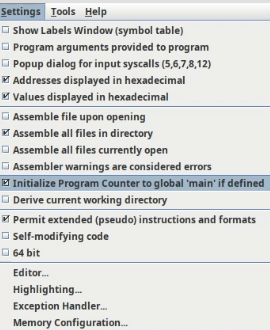
\includegraphics[width=0.4\textwidth]{img/mod-params.png}
    \caption{Установка опций <<Assemble all files in directory>> и <<Initialize Program Counter to global 'main' if defined>> для компиляции и выполнения многофайловых программ}
    \label{mod-params}
\end{figure}

%Settings -> Assemble all files in directory
%Settings -> Initialize Program Counter to global 'main' if defined

\debate[Примечание.]{Кстати, можно многофайловый проект ассемблировать и запустить, используя опции командной строки \texttt{<<p sm>>}. Они являются аналогами опций, устанавливаемых через меню.}

\section{Домашнее задание}

До 8 баллов

Написать программу, осуществляющую суммирование целочисленных элементов одномерного массива. Количество элементов в массиве может варьироваться от 1 до 10. Сами элементы вводятся с клавиатуры. Значение суммы также выводится в консоль эмулятора RARS. Необходимо контролировать, чтобы число вводимых элементов не превышало максимально допустимое. В случае, когда возникает переполнение, необходимо вывести последнее корректное значение суммы и число просуммированных при этом элементов. Суммирование осуществлять после размещения массива в памяти.

При выполнении задания для ввода и вывода массивов, вычисления суммы использовать подпрограммы, размещенные в отдельных файлах общего каталога. Для ввода и вывода отдельных элементов массива использовать макроопределения из библиотеки, рассмотренной на семинарах.

Опционально до +2 баллов

Обернуть подпрограммы ввода массива, вычисления суммы, вывода массива соответствующими макросами, используя эти макросы в основной программе вместо вызова подпрограмм. Эти макросы оформить в отдельном файле, подключаемом к основной программе вместо описания в ней глобальных точек. Подпрограммы должны также оставаться в отдельных файлах.

\textbf{\textit{Срок сдачи задания: до начала восьмого семинарского занятия в каждой из групп.}}


